\documentclass[
    DIV12,
    cleardouble=plain,
    headings=normal,
    pdftex,
    headexclude,footexclude,
    final
]{scrreprt}

\usepackage{spreadtab}
\usepackage{xspace}
\usepackage[ngerman]{babel}
\usepackage[utf8]{inputenc}
%\usepackage[T1]{fontenc}
\usepackage[pdftex]{graphicx}
\usepackage[bookmarks]{hyperref}
\usepackage{scrpage2}
\usepackage{longtable}
\usepackage{caption}
\usepackage{pgfplots}
\usepackage{float}
\usepackage{xcolor}
\usepackage{colortbl}

\graphicspath{{./}{./Pics/}}

% #################################################################

\hyphenation{Cha-otn-gsch-werl}
\setlength\headheight{1.75cm}

\ihead{\small{Hochschule Hof}}
\chead{}
\ohead{
\includegraphics[height=0.05\textheight]{fh_logo}}
\pagestyle{scrheadings}


\setcounter{secnumdepth}{5}
\setcounter{tocdepth}{5}
\renewcommand{\arraystretch}{1}

\parskip0.5\baselineskip plus 0.125\baselineskip minus 0.25\baselineskip
\parindent0em

%\automark[section]{chapter}

\titlehead{\begin{center}
\includegraphics[width=5cm]{fh_logo}\end{center}}
\title{
  Stundenplan--App für iOS \\[1em]
  Dokumentation, Spezifikation, Konstruktion
}

\author{Daniel Glaser, Stefan Scharrer, Daniel Zizer, \\ Sebastian Fuhrmann, Paul Forstern, Andreas Wolf, Kevin Rodd}
\date{06.07.2017}

% #################################################################


\begin{document}
\maketitle
\pagenumbering{roman}
\tableofcontents

%\listoftables

\newpage
\pagenumbering{arabic}

%hier die einzelnen Punkte einfügen
\chapter{Daten und Zugrifsschichten}
\section{Einleitung}
Benutzer und App-Daten werden in zwei verschiedenen Datentöpfen gespeichert. Auf bestimmte Inhalte soll nur durch die Zugriffsschichten zugegriffen werden. Im Folgenden werden die Daten und die zugehörigen Zugriffsschichten aufgelistet.\\

\begin{figure}[htb]
    \centering
    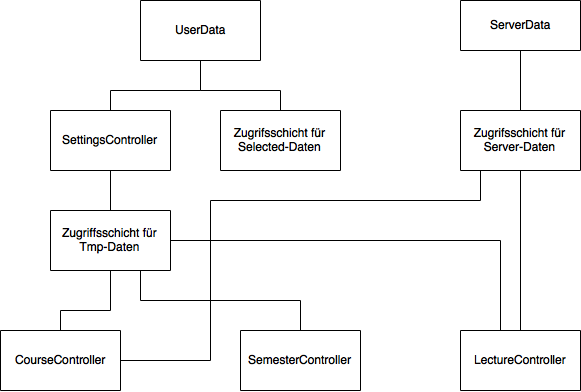
\includegraphics[width=\textwidth]{Daten}
    \caption{Daten und zugehörige Zugrifsschichten}
\end{figure}
\newpage

Folgende Datentöpfe werden genutzt:
\begin{itemize}
     \item UserData
     \item ServerData \\
\end{itemize}

Folgende Zugriffsschichten sind vorhanden:
\begin{itemize}
     \item SelectedCourse
     \item SelectedSemester
     \item SelectedLectures
     \item AllChanges
     \item AllCourses
     \item AllLectures
\end{itemize}

\newpage

\section{UserData}
Alle Daten mit relevanten Informationen über den Nutzer werden in UserData gespeichert. Mit den Zugriffsschichten SelectedLectures, SelectedSemesters, SelectedCourses und AllChanges kann auf die Daten zugegriffen, die vom User gespeichert wurden. Diese Schichten haben nur einen lesenden Zugriff und können keine Daten manipulieren. \\

Für das Ändern der Daten ist die Tmp Zugriffsschicht zuständig. Die Tmp Zugriffsschichten, welche TmpSelectedLectures, TmpSelectedSemesters und TmpSelectedCourses beinhalten, arbeiten mit einer eigenen Kopie von UserData. Dadurch können Veränderungen einfach wieder verworfen werden, da keine gespeicherten Daten verändert werden. Diese Zugriffsschichten werden nur in den Einstellungen verwendet, um u. a. die ausgewählten Studiengänge, Semester und Vorlesungen festzuhalten. Erst beim Bestätigen der Eingaben werden die Daten aus der Kopie in das original UserData übernommen. Die Kopie von UserData wird vom SettingsController erzeugt und verwaltet.\\

Im Folgenden wird der Inhalt von UserData und die zugehörigen Selected und Tmp Zugriffsschichten beschrieben.\\

In UserData sind folgende Sachen enthalten:
\begin{itemize}
     \item gewählte Season (Sommer- oder Wintersemester)
     \item gewählte Studiengänge
     \item gewählte Semester
     \item gewählte Vorlesungen
     \item Stundenplanänderungen für gewählte Vorlesungen\\     
\end{itemize}

Selected-Zugrifsschichten: 
\begin{itemize}
     \item SelectedCourse: Ist für alle vom User selektierten Studiengänge zuständig
     \item SelectedSemester: Ist für alle vom User selektierten Semester zuständig
     \item SelectedLectures: Ist für alle vom User selektierten Vorlesungen zuständig
     \item AllChanges: Ist für Änderungen von gewählte Vorlesungen zuständig \\
\end{itemize}

Tmp-Zugrifsschichten: 
\begin{itemize}
     \item TmpCourse: Ist für alle vom User selektierten Studiengänge zuständig
     \item TmpSemester: Ist für alle vom User selektierten Semester zuständig
     \item TmpLectures: Ist für alle vom User selektierten Vorlesungen zuständig
     \item AllChanges: Ist für Änderungen von gewählte Vorlesungen zuständig 
\end{itemize}

\newpage
\section{ServerData}
Alle Daten, die vom Server geladen wurden, werden in ServerData gespeichert. Durch die Zugriffsschichten AllLectures und AllCourses können die Daten abgefragt werden.

Folgend wird über die in ServerData enthaltenen Daten und die zugehörigen Zugriffsschichten informiert.

In ServerData sind folgende Sachen enthalten:
\begin{itemize}
     \item Alle Studiengänge + Semester
     \item Alle Vorlesungen für ausgewählte Studiengänge + Semester \\     
\end{itemize}

Zugriffsschichten: 
\begin{itemize}
     \item AllCourses: Ist für alle geladenen Studiengänge + Semester zuständig
     \item AllLectures: Ist für alle geladenen Vorlesungen für Studiengänge + Semester zuständig\\
\end{itemize}

\newpage
\chapter{Hintergrundaktualisierung}
\section{Einleitung}
Die App soll im Hintergrund regelmäßig prüfen, ob neue Stundenplanänderungen für den Benutzer entstanden sind.
Daher wurde der Background Fetch implementiert.
\begin{figure}[htb]
    \centering
    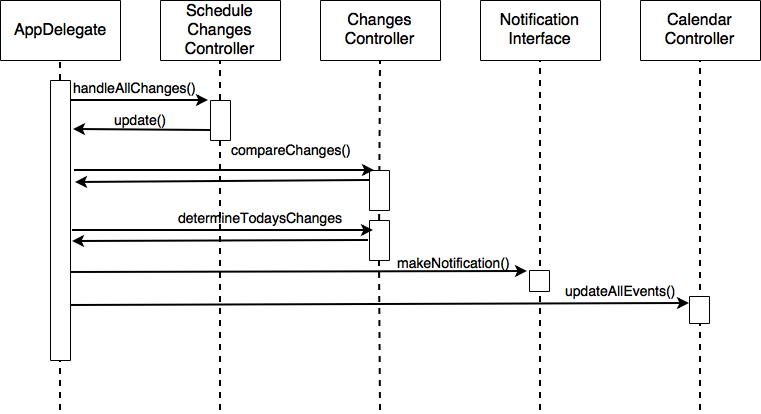
\includegraphics[width=\textwidth]{BackgroundFetch}
    \caption{Ablauf des Background Fetch}
\end{figure}

In diesem Sequenzdiagramm wird der Ablauf der application(performFetchWithCompletionHandler) Methode dargestellt. 
Zu Beginn werden durch den ScheduleChangesController die aktuellen Stundenplanänderungen vom Server geladen. 
Anschließend werden mit dem ChangesController die neu dazugekommenen Änderungen ermittelt und welche davon am aktuellen Tag stattfinden. Als Nächstes wird über das NotificationInterface eine lokale Notification für den User erstellt, die ihn über die aktuellen Stundenplanänderungen informiert.
Zuletzt wird über den CalendarController der iOS Kalender aktualisiert.

\chapter{Calendar Interface}
\begin{figure}[htb]
    \centering
    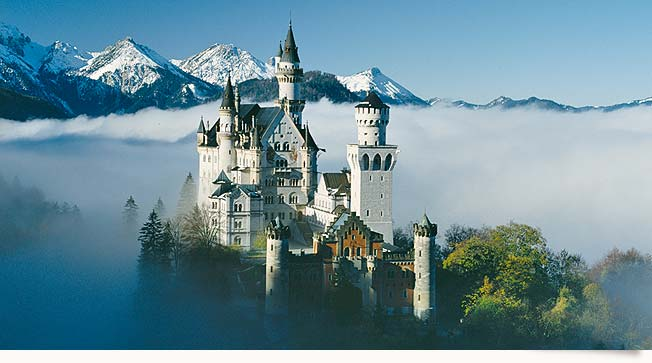
\includegraphics[height=0.3\textheight]{neuschwanstein_23}
    \caption{Diagramm}
\end{figure}
Das Calendar Interface besteht aus drei Klassen:
\begin{itemize}
     \item CalendarController
     \item CalendarInterface
     \item CalendarData
\end{itemize}

Dabei ist die CalendarController-Klasse die Klasse die aufgerufen werden muss um das Calendar Interface zu nutzen.

\section{CalendarController}
Der CalendarController ist der Controller für das Calendar Interface. Über ihm wird auf das Interface zugegriffen.


Im Folgenden wird auf die wichtigsten Methoden eingegangen:
\begin{itemize}
     \item createCalendar()
     \item removeCalendar()
     \item createAllEvents()
     \item updateAllEvents()
     \item removeAllEvents()
     \item CalendarRoutine()     
\end{itemize}

Jede Methode überprüft ob die Berechtigung gewährt wurde und reagiert entsprechend.

\subsection{createCalendar}
Erzeugt den Kalender falls die Berechtigung vorhanden ist. Falls er erzeugt wurde werden die Events mit createAllEvents in den Kalender geschrieben. Als Rückgabewert gibt er den Berechtigungsstatus zurück. Es gibt drei Rückgabewerte:
\begin{itemize}
     \item authorized \\[0.5em]
     Bedeutet das der Nutzer die Berechtigung erteilt hat und der Kalender angelegt wurde oder bereits angelegt war.
     \item notDetermined \\[0.5em]
     Bedeutet das die Berechtigung gerade abgefragt wird.
     \item denied \\[0.5em]
     Bedeutet das die Berechtigung verweigert wurden.
\end{itemize}

\subsection{removeCalendar}
Löscht den Kalender mit Hilfe des CalendarInterface.

\subsection{createAllEvents}
Erzeugt die aus den Vorlesungen die Events, die anschließend mit Hilfe des CalendarInterface in den Kalender geschrieben werden.
Falls der Kalender noch nicht erzeugt wurde wird er angelegt.
Die EventID's werden persistent gespeichert.

\subsection{updateAllEvents}
Ermittelt welche Art von Änderung vorliegt und passt die Events mit Hilfe des CalendarInterface entsprechend an.
Die EventID's werden persistent gespeichert.

\subsection{removeAllEvents}
Holt sich für die übergebenden Vorlesungen die EventID's und löscht die entsprechenden Events mit Hilfe des CalendarInterface.
Die Änderungen an den EventID's werden persistent gespeichert.

\subsection{CalendarRoutine}
Aktualisiert die Vorlesungen im Kalender. Dazu holt sie sich die abgewählten und neu ausgewählten Vorlesungen und übergibt sie der removeAllEvents oder createAllEvents-Methode.

\section{CalendarInterface}
Dies ist die Klasse die direkt auf den Kalender zugreift. 

Im Folgenden wird auf die wichtigsten Methoden eingegangen:
\begin{itemize}
     \item createCalenderIfNeeded()
     \item removeCalendar()
     \item createEvent()
     \item updateEvent()
     \item removeEvent()
     \item saveIDs()
\end{itemize}

\subsection{createCalenderIfNeeded}
Erzeugt den Kalender falls er nicht bereits vorhanden ist. Gibt einen Boolean-Wert zurück ob der Kalender angelegt wurde.

\subsection{removeCalendar}
Löscht den Kalender falls dieser vorhanden ist. Gibt einen Boolean-Wert zurück ob das Löschen erfolgreich war.

\subsection{createEvent}
Schreibt das übergebende Event in den Kalender.

\subsection{updateEvent}
Das zu der EventID dazugehörige Event wird mit den entsprechend Werten des übergebenen Event angepasst.

\subsection{removeEvent}
Löscht das übergebene Event. Gibt einen Boolean-Wert zurück ob das Löschen erfolgreich war.

\subsection{saveIDs}
Speichert die EventIDs der Vorlesungen und Änderungen.

\section{CalendarData}
Die CaledenarData-Klasse dient dazu, die EventIDs der Vorlesungen und Änderungen getrennt in Dictonarys zu speichern.
Die Dictonarys bestehen aus einer Zuordnung von einer ID einer Vorlesung zu mehreren EventIDs.


\chapter{Date Extension}
Die DateExtension enthält Methoden zur Erweiterung der Date Klasse.

Im Folgenden werden die wichtigsten Methoden der Klasse aufgelistet.
\begin{itemize}
     \item checkSemester() -$>$ String
     \item startSemester(semester : String) -$>$ Date
     \item endSemester(semester : String) -$>$ Date
     \item startLecture(startDate: Date, weekdayString : String, semester : String) -$>$ Date
     \item endLecture (endDate: Date, weekdayString : String, semester : String) -$>$ Date
     \item calendarweekToDate(day: String, cw: Int, date: Date) -$>$ Date   
     \item combineDateAndTime(date: Date, time: Date) -$>$ Date
     \item changeStartFromTwoWeekLecture()
\end{itemize}
\newpage

\section{checkSemester() -$>$ String}
Überprüft und gibt danach einen String zurück, ob das momentane Semester ein Sommersemester oder Wintersemester ist. 

\section{startSemester(semester : String) -$>$ Date}
Gibt das Startdatum des aktuellen Semesters zurück. Wenn das Startdatum im Sommersemester (15.03) oder im Wintersemester (01.10) ein Freitag, Samstag oder Sonntag ist, beginnt die Vorlesung am nächstfolgenden Montag.

\section{endSemester(semester : String) -$>$ Date}
Gibt das Enddatum des aktuellen Semesters zurück. Wenn das Enddatum im Sommersemester (10.07) oder im Wintersemester (25.01) ein Samstag, Sonntag oder Montag ist endet, die Vorlesung am vorausgehenden Freitag.

\section{startLecture(startDate: Date, weekdayString : String, semester : String) -$>$ Date}
Gibt das Startdatum der Vorlesung zurück. Das Startdatum wird mittels des Starts des Semesters und dem Wochentag der Vorlesung ermittelt.

\section{endLecture (endDate: Date, weekdayString : String, semester : String) -$>$ Date}
Gibt das Enddatum der Vorlesung zurück. Das Enddatum wird mittels des Endes des Semesters und dem Wochentag der Vorlesung ermittelt.

\section{calendarweekToDate(day: String, cw: Int, date: Date) -$>$ Date}
Ermittelt aus einer Kalenderwoche und dem dazugehörigen Wochentag ein Datum.

\section{combineDateAndTime(date: Date, time: Date) -$>$ Date}
Kombiniert das Datum und die Uhrzeit von zwei verschiedenen Daten.

\section{changeStartFromTwoWeekLecture(startDate: Date, semester: String) -$>$ Date}
Ändert das Startdatum einer Vorlesung die alle zwei Wochen stattfindet.
\chapter{Artificial Intelligence}
Die Artificial Intelligence enthält Methoden, die das Kommentar der jeweiligen Vorlesung überprüft. Falls es im Kommentar enthalten ist, erkennt sie ob die Vorlesung ein Blocktermin ist, alle zwei Wochen stattfindet, eine Aufzählung von Terminen enthält, nicht parsbar ist, wann die Vorlesung beginnt oder wann sie endet. Die Artificial Intelligence wird direkt aufgerufen, nachdem die Vorlesung in der Klasse JsonLecture vom Server abgefragt werden.

Im Folgenden werden die wichtigsten Methoden der Klasse aufgelistet.
\begin{itemize}
     \item iterationOfLecture(comment: String, start: Date, end: Date) -$>$ iterationState
     \item containsEnumeration(comment: String) -$>$ Bool
     \item checkPeriod(comment: String) -$>$ (String, String)
     \item checkStart(comment: String) -$>$ String
     \item checkEnd(comment: String) -$>$ String
     \item getNextCalendarWeekOrDate(comment: String, keyword: String, length: Int) -$>$ String     
     \item getPreviousCalendarWeekOrDate(comment: String, keyword: String, length: Int) -$>$ String
\end{itemize}

\section{iterationOfLecture(comment: String, start: Date, end: Date) -$>$ iterationState}
Gibt die verschiedenen Arten der Wiederholung einer Vorlesung zurück. Es gibt fünf verschiedene Rückgabewerte.
\begin{itemize}
     \item iterationState.notParsable  \\[0.5em]
     Bedeutet, dass das Kommentar Wörter enthält die das Programm nicht parsen kann.
     \item iterationState.calendarWeeks \\[0.5em]
     Bedeutet, dass das Kommentar eine Aufzählung von Terminen enthält.
     \item iterationState.individualDate \\[0.5em]
     Bedeutet, dass die Vorlesung ein Einzeltermin ist.
     \item iterationState.twoWeeks \\[0.5em]
     Bedeutet, dass die Vorlesung alle zwei Wochen stattfindet.
     \item iterationState.weekly \\[0.5em]
     Bedeutet, dass die Vorlesung jede Wochen stattfindet.
\end{itemize}

\section{containsEnumeration(comment: String) -$>$ Bool}
Falls das Kommentar eine Aufzählung von Terminen enthält gibt die Methode diese zurück.

\section{checkPeriod(comment: String) -$>$ (String, String)}
Durchsucht das Kommentar nach einer Zeitspanne. Ein Beispiel so einer Zeitspanne ist "KW 12 bis 26", dabei wird die erste Kalenderwoche als Starttermin und die zweite als Endtermin der Vorlesung genommen. Vorerst sucht es jedoch nach Zeitspannen die nichts mit den Vorlesungsterminen zu tun haben, beispielsweise "Online-Anmeldung 09.03. - 16.03.", und entfernt diese temporär aus dem Kommentar.

\section{checkStart(comment: String) -$>$ String}
Durchsucht das Kommentar nach einem neuen Startdatum der Vorlesung.

\section{checkEnd(comment: String) -$>$ String}
Durchsucht das Kommentar nach einem neuen Enddatum der Vorlesung.

\section{getNextCalendarWeekOrDate(comment: String, keyword: String, length: Int) -$>$ String}
Gibt das nächste Datum oder die nächste Kalenderwoche nach dem angegebenen Keyword zurück. Length gibt dabei die Länge an wie viel Zeichen die Methode nach dem Keyword suchen soll, bevor sie die Suche nach einem Datum oder einer Kalenderwoche abbricht.

\section{getPreviousCalendarWeekOrDate(comment: String, keyword: String, length: Int) -$>$ String}
Gibt das vorrausgehende Datum oder die vorrausgehende Kalenderwoche nach dem angegebenen Keyword zurück. Length gibt dabei an, welche Anzahl an Zeichen die Methode vor dem Keyword suchen soll, bevor sie die Suche nach einem Datum oder einer Kalenderwoche abbricht.
\documentclass[a4paper, 12pt]{article}

\usepackage[ngerman]{babel}
\usepackage[utf8]{inputenc}

\usepackage{graphicx}
\pagestyle{headings}
\author{Author: Kevin Rodd}
\title{iOS Job-Manager}


\begin{document}

\thispagestyle{empty}
\begin{center}
\Large{Hochschule für Angewandte Wissenschaften Hof}\\
\end{center}


\begin{center}
\Large{Fachbereich Informatik}
\end{center}
\begin{verbatim}





\end{verbatim}
\begin{center}
\textbf{\LARGE{iOS JobManager}}
\end{center}
\begin{verbatim}


\end{verbatim}
\begin{center}
\textbf{im Studiengang Mobile Computing}
\end{center}
\begin{verbatim}
\end{verbatim}

\begin{flushleft}
\begin{tabular}{lll}
\textbf{Thema:} & & Allgemeine Funktionsweise und Ablauf des JobManagers \\

& & \\
& & \\
\textbf{verfasst von:} & & Kevin Rodd \flq{}kevin.rodd@hof-university.de\frq{}\\
& & \\
& & \\
\end{tabular}
\end{flushleft}


\newpage

\tableofcontents

\newpage

\section{Einleitung}
\begin{figure}
	\centering
	\includegraphics[scale=0.6]{JobManager.png}
	\caption{Architektur und Integration des JobManagers in die Stundenplan App}
	\label{img:JobManager-Architektur}
\end{figure}
Im folgenden Dokument, wird auf die Funktionsweise des JobManagers in der iOS Stundenplan App der Hochschule Hof näher eingegangen.
\newline Innerhalb der Applikation verwaltet der JobManager alle Jobanfragen und delegiert die Aufgaben asynchron an die jeweils unterliegende Schicht.
\newline
\newline Jede Instanz des JobMangers verwaltet seine eigene Warteschlange (Queue). In dieser Warteschlange können sich n Workitems befinden. Jedes Workitem stellt eine Netzwerkanfrage (einen Job) dar. Ergebnisse werden in der Warteschlange gesammelt und sobald alle Ergebnisse vorliegen, werden diese an den Auftraggeber weitergegeben.
\newline
Eine Abbruchfunktion für noch offene Jobs lässt den Vorgang jederzeit unterbrechen.
\newpage
\section{Ablauf}
Der Ablauf des JobManagers und die Verwendung für den Benutzer lässt sich in folgende Unterpunkte unterteilen:
\newline
\subsection{Erstellen des JobManagers}
Der JobManager wird ohne speziellen Konstruktor erstellt. Dazu reicht ein 
\newline  \textit{var myJobManager : JobManager = JobManager()}.

\subsection{Observer anmelden}
Ebenso ist das Anmelden des Observers schnell erledigt. Hierzu muss der jeweilige Controller lediglich das \textit{DataObserverProtocol}  implementieren und mittels
\newline
\newline
\textit{self.myJobManager.addNewObserver(o: self)}
\newline
\newline sich beim JobManager als Observer anmelden.

\subsection{Anfrage}
Wurde der JobManager erstellt und man hat sich als Observer angemeldet, so kann man eine neue Jobanfrage an den JobManager stellen. Eine Anfrage könnte so aussehen:
\newline
\newline \textit{myJobManager.NetworkJob(url: urlString, username: myUsername, password: myPassword)}
\newline
\newline Hier ist zu beachten, dass das einfügen eines Usernames und eines Passwortes optionale Parameter sind. 

\subsection{Ergebnis}
Sind alle Jobs erfolgreich beendet worden, so sendet der JobManager die Daten als \textit{AnyObject} an die update(o: AnyObject) Methode des Oberservers. 
\newline
\subsection{Aktuelle Version}
In der aktuellen Version ist es möglich den JobManger mehrmals zu verwenden. Eine neue Instanziierung ist nicht notwendig, wird jedoch für einen sauberen Ablauf empfohlen.

\newpage



\end{document}


\end{document}
